\documentclass[twoside,openright,titlepage,fleqn,
	headinclude,11pt,a4paper,BCOR5mm,footinclude
	]{scrbook}
%--------------------------------------------------------------
        \newcommand{\myTitle}{Progettazione e Analisi di Algoritmi\xspace}
% use the right myDegree option
\newcommand{\myDegree}{Corso di Laurea Magistrale in Informatica\xspace}
%\newcommand{\myDegree}{
	%Corso di Laurea Specialistica in Scienze e Tecnologie 
	%dell'Informazione\xspace}
\newcommand{\myName}{Massimo Nocentini\xspace}
\newcommand{\myProf}{Donatella Merlini\xspace}
\newcommand{\myOtherProf}{Maria Cecilia Verri\xspace}
\newcommand{\mySupervisor}{Nome Cognome\xspace}
\newcommand{\myFaculty}{
	Facolt\`a di Scienze Matematiche, Fisiche e Naturali\xspace}
\newcommand{\myDepartment}{
	Dipartimento di Sistemi e Informatica\xspace}
\newcommand{\myUni}{\protect{
	Universit\`a degli Studi di Firenze}\xspace}
\newcommand{\myLocation}{Firenze\xspace}
\newcommand{\myTime}{Anno Accademico 2012-2013\xspace}
\newcommand{\myVersion}{Version 0.1\xspace}

%--------------------------------------------------------------
\usepackage[latin1]{inputenc} 
\usepackage[T1]{fontenc} 
\usepackage[square,numbers]{natbib} 
\usepackage[fleqn]{amsmath}  
\usepackage[english]{babel}
\usepackage{ae,aecompl}
\usepackage[pdftex]{graphicx}
\usepackage{latexsym}
\usepackage{amsmath, amsthm, amssymb}
\usepackage{rotating}
\usepackage{boxedminipage}
\usepackage{multicol}
\usepackage{rotating}

%--------------------------------------------------------------
\usepackage{dia-classicthesis-ldpkg} 
%--------------------------------------------------------------
% Options for classicthesis.sty:
% tocaligned eulerchapternumbers drafting linedheaders 
% listsseparated subfig nochapters beramono eulermath parts 
% minionpro pdfspacing
\usepackage[eulerchapternumbers,subfig,beramono,eulermath,
	parts]{classicthesis}
%--------------------------------------------------------------
\newlength{\abcd} % for ab..z string length calculation
% how all the floats will be aligned
\newcommand{\myfloatalign}{\centering} 
\setlength{\extrarowheight}{3pt} % increase table row height
\captionsetup{format=hang,font=small}
%--------------------------------------------------------------
% Layout setting
%--------------------------------------------------------------
\usepackage{geometry}
\geometry{
	a4paper,
	ignoremp,
	bindingoffset = 1cm, 
	textwidth     = 13.5cm,
	textheight    = 21.5cm,
	lmargin       = 3.5cm, % left margin
	tmargin       = 4cm    % top margin 
}
%--------------------------------------------------------------
\usepackage{listings}
\usepackage{hyperref}
\usepackage{pdfpages}
% My Theorem
\newtheorem{oss}{Observation}[section]
\newtheorem{exercise}{Exercise}[section]
\newtheorem{thm}{Theorem}[section]
\newtheorem{cor}[thm]{Corollary}

\newtheorem{lem}[thm]{Lemma}

\newcommand{\vect}[1]{\boldsymbol{#1}}

% questo comando e' relativo alle correzioni che puo
% apportare il prof se lo desidera.
\newcommand{\prof}[1]{\boldsymbol{#1}}

% instead of boldsymbol I can use the arrow above the letter with
%\newcommand{\vect}[1]{\vec{#1}}

% page settings
% \pagestyle{headings}
%--------------------------------------------------------------
\begin{document}
\frenchspacing
\raggedbottom
\pagenumbering{roman}
\pagestyle{plain}
%--------------------------------------------------------------
% Frontmatter
%--------------------------------------------------------------
%--------------------------------------------------------------
% titlepage.tex (use thesis.tex as main file)
%--------------------------------------------------------------
\begin{titlepage}
	\begin{center}
   	\large
      \hfill
      \vfill
      \begingroup
			\spacedallcaps{\myUni} \\ 
			\myFaculty \\
			\myDegree \\ 
			\vspace{0.5cm}
         
\includegraphics[scale=.065]{logo/unifi}\\
         \vspace{0.5cm}    
         %% -------put here the type of document---ie: Tesi di Laurea
         Elaborato d'Esame
      \endgroup 
      \vfill 
      \begingroup
      	\color{Maroon}\spacedallcaps{\myTitle} \\ \bigskip
      \endgroup
      \spacedlowsmallcaps{\myName}
      \vfill  
      % Professoresse:
      \itshape{\myProf}\\\itshape{\myOtherProf}
      \vfill  
      \myTime
      \vfill                      
	\end{center}        
\end{titlepage}   
%--------------------------------------------------------------
% back titlepage
%--------------------------------------------------------------
   \newpage
	\thispagestyle{empty}
	\hfill
	\vfill
	\noindent\myName: 
	\textit{\myTitle,} 
	\myDegree, \textcopyright\ \myTime
%--------------------------------------------------------------
% back titlepage end
%--------------------------------------------------------------
\pagestyle{scrheadings}
%--------------------------------------------------------------
% Mainmatter
%--------------------------------------------------------------
\pagenumbering{arabic}

% settings for the lstlisting environment
\lstset{
	language = R
	, numbers = left 
	, basicstyle=\sffamily%\footnotesize
%	, frame=single
	, tabsize=2
	, captionpos=b
	, breaklines=true
	, showspaces=false
	, showstringspaces=false
}

\tableofcontents

\newpage

\newpage

\subsection*{Text contents}
All the text content is distributed under:\\
\textbf{ This work is licensed under the Creative Commons Attribution,
  NonCommercial, ShareAlike 3.0 Unported License. To view a
  copy of this license, visit\\
  \href{http://creativecommons.org/licenses/by-nc-sa/3.0/}{http://creativecommons.org/licenses/by-nc-sa/3.0/}\\
  or send a letter to Creative Commons, 444 Castro Street, Suite 900,
  Mountain View, California, 94041, USA.}

\begin{center}

\includegraphics{cc-icons-eps/by}

\includegraphics{cc-icons-eps/cc}

\includegraphics{cc-icons-eps/nc}

\includegraphics{cc-icons-eps/sa}
\end{center}

\subsection*{Sources}
All sources are distributed under, where the word ``Software'' is
referred to all of the sources that are present in this work: \\
\textbf{
  Copyright (c) 2011 Massimo Nocentini\\
  Permission is hereby granted, free of charge, to any person
  obtaining a copy of this software and associated documentation files
  (the "Software"), to deal in the Software without restriction,
  including without limitation the rights to use, copy, modify, merge,
  publish, distribute, sublicense, and/or sell copies of the Software,
  and to permit persons to whom the Software is furnished
  to do so, subject to the following conditions:\\
  The above copyright notice and this permission notice shall be
  included in all
  copies or substantial portions of the Software.\\
  THE SOFTWARE IS PROVIDED "AS IS", WITHOUT WARRANTY OF ANY KIND,
  EXPRESS OR IMPLIED, INCLUDING BUT NOT LIMITED TO THE WARRANTIES OF
  MERCHANTABILITY, FITNESS FOR A PARTICULAR PURPOSE AND
  NONINFRINGEMENT. IN NO EVENT SHALL THE AUTHORS OR COPYRIGHT HOLDERS
  BE LIABLE FOR ANY CLAIM, DAMAGES OR OTHER LIABILITY, WHETHER IN AN
  ACTION OF CONTRACT, TORT OR OTHERWISE, ARISING FROM, OUT OF OR IN
  CONNECTION WITH THE SOFTWARE OR THE USE OR OTHER DEALINGS IN THE
  SOFTWARE.  }


\part{Analysis part}

\chapter{Lectures notes}
\section{Sorting algorithms}

We study two algorithms that are based on checks between keys, those
are MERGESORT and QUICKSORT.

\subsection{MERGESORT algorithm}

The MERGESORT algorithm is independent from keys present in the
input vector and it behaves the same regardless the given input.
Let $n = 2^m$ be the length of the vector to be ordered, we define a
function $C$ which count the number of checks needed to order the
input vector. $C$ definition strictly follows the algorithmic method:
\begin{displaymath}
  C(2^m) = 2C(2^{m-1}) + 2^m
\end{displaymath}
Solving the recurrence\footnote{put here the proof} we get $C(n)
\in O(n logn)$: observe that if we use an algorithm based on checks
between keys, it isn't possible to do better than to build a ``checks tree'',
hence we've found
a lower bound for the complexity of this class of algorithms \footnote{in
  the slides of the first lecture maybe there's more material about
  this topic}.

\subsection{QUICKSORT algorithm}
The QUICKSORT algorithm depends on the distribution of the keys in the
input vector. For what follow we assume to have a probability space
$\Omega = D_n$, where $D_n$ is the set of permutation of length $n$
without repetition over $\{1,\ldots,n\}$. We focus on the simpler
variant where the pivot is chosen as the right-most
key\footnote{report here the code}.  We study the behavior of an
application to the vector $\left ( 20, 25, 7, 3, 30, 8, 41,
  18\right)$, \autoref{tab:quicksort-example} reports performed steps.
\begin{table}[ht]
  \caption{Quicksort example}
  \label{tab:quicksort-example}
  \begin{center}
    \begin{tabular}{cccccccccc}
      20 & 25 & 7 & 3 & 30 & 8 & 41 & 18 &  &  \\
      $\uparrow i$ & & & & & $\uparrow j$ & & $\uparrow pivot$ &
      $\rightarrow$ & $\{20, 41, 8\}$ \\
      8 & 25 & 7 & 3 & 30 & 20 & 41 & 18 &  &  \\
       & $\uparrow i$ & & $\uparrow j$ & &  & & $\uparrow pivot$ &
       $\rightarrow$ & $\{25, 30, 3\}$ \\
       8 & 3 & 7 & 25 & 30 & 20 & 41 & 18 &  &  \\
       &  & $\uparrow j$ & $\uparrow i$ & &  & & $\uparrow pivot$ &
       $\rightarrow$ & $\{7, 25, 7\}$ \\
       8 & 3 & 7 & 18 & 30 & 20 & 41 & 25 &  &  \\
       &  &  & $\uparrow pivot$ & &  & &  &
       $\rightarrow$ & recursion \\
    \end{tabular}
  \end{center}
\end{table}
Observe that in order to move the $pivot$ element in its final
position, it is necessary for two keys ($7, 25$) to be checked
twice against the $pivot$, moreover when the second of those checks
happens, indexes $i$ and $j$ overlapped at some time such that $j < i$
eventually holds.

Hence, given a vector of length $n$, the number of checks
performed before recurring on left and right partitions is $(n-1) + 2$,
where $n-1$ appears because the $pivot$ element isn't indexed neither with
$i$ nor with $j$.  We analyze the number of performed checks by cases:

\begin{description}
\item[worst case] when the vector is already ordered, in either one of the
  two directions, recursion works over one partition only because the
  other one has to be empty, hence the number of checks satisfies
  the following relation:
  \begin{displaymath}
    C(n) = (n-1)+2 + C(n-1)
  \end{displaymath}
  Unfolding $C(n-1)$ and fixing $C(0) = 0$ as base case, the following holds:
  \begin{displaymath}
    \begin{split}
      C(n) &= (n+1) + C(n-1) = (n+1) + n + C(n-2) = \\
      &= (n+1) + n + (n-1) + \ldots + 2 + C(0) = \\
      &= \sum_{k=2}^{n+1}{k} + C(0) = \sum_{k=1}^{n+1}{k} -1 + C(0) =
      \frac{(n+1)(n+2)}{2} - 1
    \end{split}
  \end{displaymath}
  so $C(n) \in O(n^2)$.
\item[best case] when the partition phase puts the $pivot$ element
    in the middle then QUICKSORT recurs on balanced partitions. In this
  case it has the same complexity of MERGESORT, hence $C(n) \in O(n
  logn)$
\end{description}
We explain the average case in the following dedicated section.

\subsection{QUICKSORT: On the average number of checks}

To study this case we have to consider all
elements of $\Omega$ (recall that $w \in \Omega \rightarrow (w[i]\in
\{1,\ldots,n\}) \wedge (\forall i\not =j: w[i]\not=w[j])$). First of
all we can suppose that $j$ is the $pivot$, hence a generic $w$ will
have this structure:
\begin{displaymath}
  w = (C_{j-1} \quad C_{n-j} \quad j)
\end{displaymath}
where $C_k$ is a vector of length $k$. We can consider the
probability to have $j$ as $pivot$ considering the uniform
distribution on $\Omega$:
\begin{displaymath}
  \mathbb{P}\left(w\in\Omega: w[n]=j \right) =
  \frac{(n-1)!}{n!} =  \frac{1}{n}
\end{displaymath}
Our goal here is to build a function $C(n)$ which counts the average
number of checks during an execution of the algorithm given an input
vector of length $n$. In order to do that observe that every keys $j
\in \{1,\ldots,n\}$ can be the $pivot$, we can write:
\begin{displaymath}
  C(n) = (n+1) +  \frac{1}{n}\sum_{j=1}^{n}{C(j-1) + C(n-j)}
\end{displaymath}
Observing the sum when $j$ runs:
\begin{displaymath}
  \begin{split}
    j=1 &\rightarrow C(0) + C(n-1) \\
    j=2 &\rightarrow C(1) + C(n-2) \\
    \ldots& \\
    j=n-1 &\rightarrow C(n-2) + C(1) \\
    j=n &\rightarrow C(n-1) + C(0) \\
  \end{split}
\end{displaymath}
Hence we can rewrite:
\begin{displaymath}
  C(n) = (n+1) +  \frac{2}{n}\sum_{j=0}^{n-1}{C(j)}
\end{displaymath}
Now we do some manipulation:
\begin{displaymath}
  \begin{split}
    C(n) &= (n+1) + \frac{2}{n}\sum_{j=0}^{n-1}{C(j)}\\
    nC(n) &= n(n+1) + 2\sum_{j=0}^{n-1}{C(j)}
  \end{split}
\end{displaymath}
Subtract the previous $(n-1)$ term to both members:
\begin{displaymath}
  \begin{split}
    nC(n) -(n-1)C(n-1) &= n(n+1) + 2\sum_{j=0}^{n-1}{C(j)} \\
    &-\left((n-1)((n-1)+1) + 2\sum_{j=0}^{(n-1)-1}{C(j)}\right) \\
    % nC(n) -(n-1)C(n-1)
    &= n(n+1) + 2\sum_{j=0}^{n-1}{C(j)} \\
    &-n(n-1) - 2\sum_{j=0}^{n-2}{C(j)} \\
    &= n(n+1-(n-1)) + 2C(n-1) \\
    &= 2(n + C(n-1)) \\
  \end{split}
\end{displaymath}
Getting $nC(n) = 2n + (n+1)C(n-1)$, divide both member by $n(n+1)$:
\begin{displaymath}
  \begin{split}
    \frac{C(n)}{n+1}  = \frac{2}{n+1} +
    \frac{C(n-1)}{n}
  \end{split}
\end{displaymath}
We arrived at a recurrence $A(n) = b(n) + A(n-1)$, where $A(n) =
\frac{C(n)}{n+1} $ and $b(n) = \frac{2}{n+1} $. So we expand, fixing
$C(0) = 0$:
\begin{displaymath}
  \begin{split}
    \frac{C(n)}{n+1} &= \frac{2}{n+1} + \frac{C(n-1)}{n} =
    \frac{2}{n+1} +
    \frac{2}{n} + \frac{C(n-2)}{n-1}\\
    &= \frac{2}{n+1} + \frac{2}{n} + \ldots +
    \frac{2}{3} + \frac{2}{2} + \frac{C(0)}{1}\\
    &= \frac{2}{n+1} + \frac{2}{n} + \ldots +
    \frac{2}{3} + 1\\
    &= 2\left(\frac{1}{n+1} + \frac{1}{n} + \ldots +
      \frac{1}{3}\right) + 1\\
    &= 2\left(\frac{1}{n+1} + \frac{1}{n} + \ldots +
      \frac{1}{3}\right) +2\frac{1}{2} + 2
    + 1 -2\frac{1}{2} - 2\\
    &= 2\left(\frac{1}{n+1} + \frac{1}{n} + \ldots +
      \frac{1}{3}+
      \frac{1}{2}+
      1\right) -2 \\
    &= 2(H_{n+1}-1)
  \end{split}
\end{displaymath}
Having recognized the harmonic numbers $H_{n+1}=\left(\frac{1}{n+1} +
  \frac{1}{n} + \ldots + \frac{1}{3}+ \frac{1}{2}+ 1\right)$, the
final result is $$C(n) = 2(n+1)(H_{n+1}-1)$$

In order to bound $C(n)$ we have to recall that $H_n \sim ln(n) +
\gamma$, hence $C(n) \in O(nlogn)$.

From a practical point of view, to avoid the worst case, when a
sorting problem is approached with the QUICKSORT algorithm we can
choose to do one of the following actions before starting the sorting
process:
\begin{itemize}
\item shuffling the input vector and proceed with the algorithm
  described above;
\item choose the $pivot$ element at random, move it in the right-most
  position and proceed with the algorithm described above.
\end{itemize}
Each of the two tricks require linear time in the dimension of the
input vector and allow us to use the result of the average case and
working with $O(nlogn)$ number of checks.

\subsection{QUICKSORT: On the average number of swaps}
Our goal here is to build a function $S(n)$ which counts the average
number of swaps during an execution of the algorithm given an input
vector of length $n$.

The recurrence for the average number of swaps is as follow:
\begin{displaymath}
  S(n) =  \frac{n-2}{6} +  \frac{1}{n} \sum_{j=1}^{n}{S(j-1) + S(n-j)}
\end{displaymath}
We proceed the proof in two stages, first studying
\begin{displaymath}
  one: \mathbb{E} \left[K_j \right]  = \frac{(j-1)(n-j)}{n-1}
\end{displaymath}
where $K_j$ is a random variable that depends on $j$, after
\begin{displaymath}
  two: \frac{n-2}{6} = \frac{1}{n}\sum_{j=1}^{n}{
    \mathbb{E} \left[K_j \right] }
\end{displaymath}
In what follow, suppose to have a probability space $\Omega$ as
defined in the previous sections and an uniform distribution above it.
\begin{proof}[Proof of $one$]
  Again, suppose the $pivot$ is $j \in \left \lbrace
    1,\ldots,n \right\rbrace $. We define the random variable $K_j:
  \Omega \rightarrow \mathbb{R}$ such that:
  \begin{displaymath}
    \begin{split}
      w[n] = j &\rightarrow K_j(w) = s \\
      w[n] \not= j &\rightarrow K_j(w) = 0 \\
    \end{split}
  \end{displaymath}
  where $s$ is the number of swaps performed by the partitioning phase
  of QUICKSORT given an input vector $w$ of length $n$ (hence the
  variable $K_j$ counts the number of swaps). Now we can compute the
  probability to have $k$ swaps when $j$ is the $pivot$:
  \begin{displaymath}
    \mathbb{P}\left(K_j = k \right) =  \frac{{{n-j}\choose{k}}
      {{j-1}\choose{k}} (n-j)! (j-1)! }{(n-1)!}
  \end{displaymath}
  We can justify the above formula in the following steps:
  \begin{itemize}
  \item we have $k$ swaps when $\left| \left \lbrace
        w_i : w_i < j \right\rbrace \right| = k$ and
    $\left| \left \lbrace
        w_i : w_i > j \right\rbrace \right| = k$
  \item we can choose $k$ keys from $\left \lbrace w_i : w_i < j
    \right\rbrace$ in ${{j-1}\choose{k}}$ ways and, for each choice,
    there are $(j-1)!$ ways to sort them;
  \item we can choose $k$ keys from $\left \lbrace w_i : w_i > j
    \right\rbrace$ in ${{n-j}\choose{k}}$ ways and, for each choice,
    there are $(n-j)!$ ways to sort them;
  \item the total number of possible permutation of $n$ keys excluding
    the $pivot$ (which is fixed in the right-most position) is
    $(n-1)!$
  \end{itemize}
  Now we study the mean of the variable $K_j$:
  \begin{displaymath}
    \mathbb{E} \left[ K_j \right] = \sum_{k \geq 0}{k \mathbb{P}\left(
        K_j = k      \right) }
  \end{displaymath}
  Using ${{n}\choose{m}} =  \frac{n!}{m!(n-m)!} $, we can rewrite:
  \begin{displaymath}
    \mathbb{P}\left(K_j = k \right) =  {{n-j}\choose{k}}
    {{j-1}\choose{k}} \frac{(n-j)! (j-1)! }{(n-1)!} =  {{n-j}\choose{k}}
    {{j-1}\choose{k}} {{n-1}\choose{j-1}}^{-1}
  \end{displaymath}
  We put the previous rewrite of $\mathbb{P}\left(K_j = k \right)$ into
  the definition of $\mathbb{E} \left[ K_j \right]$:
  \begin{displaymath}
    \mathbb{E} \left[ K_j \right] = \sum_{k \geq 0}{k \mathbb{P}\left(
        K_j = k      \right) }  = \sum_{k \geq 0}{k \frac{{{n-j}\choose{k}}
        {{j-1}\choose{k}}}{{{n-1}\choose{j-1}}}}
  \end{displaymath}
  Using the following rewrite for ${{j-1}\choose{k}}$:
  \begin{displaymath}
    {{j-1}\choose{k}} =  \frac{(j-1)!}{k!(j-1-k)!} =
    \frac{(j-1)}{k} \frac{(j-2)!}{(k-1)!(j-1-k)!} =
    \frac{(j-1)}{k}{{j-2}\choose{k-1}}
  \end{displaymath}
  And ${{n}\choose{m}} = {{n}\choose{n-m}}$ implies ${{j-2}\choose{k-1}}
  = {{j-2}\choose{j-2 -(k-1)}} = {{j-2}\choose{j -k-1}}$, then:
  \begin{displaymath}
    \begin{split}
      \mathbb{E} \left[ K_j \right] &= \sum_{k \geq 0}{k
        \mathbb{P}\left( K_j = k \right) } =
      \frac{1}{{{n-1}\choose{j-1}}} \sum_{k \geq 0}{k
        {{n-j}\choose{k}} {{j-1}\choose{k}}} \\
      &= \frac{1}{{{n-1}\choose{j-1}}} \sum_{k \geq 0}{k
        {{n-j}\choose{k}}  \frac{j-1}{k}{{j-2}\choose{j-k-1}}}
      = \frac{j-1}{{{n-1}\choose{j-1}}} \sum_{k \geq 0}{
        {{n-j}\choose{k}} {{j-2}\choose{j-k-1}}}
    \end{split}
  \end{displaymath}
  Now we recognize the Vandermonde result:
  \begin{displaymath}
    \sum_{k \geq 0}{{{r}\choose{k}} {{s}\choose{n-k}}  } =
    {{r + s}\choose{n}}
  \end{displaymath}
  which can be proved directly because the ipergeometric distribution
  has exactly the same structure, and being a distribution, it sum up
  to 1. So we use this result applying it to $\sum_{k \geq 0}{
    {{n-j}\choose{k}} {{j-2}\choose{j-k-1}}} = {{n-2}\choose{j-1}} $,
  obtaining:
  \begin{displaymath}
    \begin{split}
      \mathbb{E} \left[ K_j \right] &= \frac{j-1}{{{n-1}\choose{j-1}}}
      {{n-2}\choose{j-1}} =
      \frac{(j-1)(n-2)!(j-1)!(n-j)!}{(n-1)!(j-1)!(n-j-1)!}=\\
      &=\frac{(j-1)(n-2)!(j-1)!(n-j)(n-j-1)!}
      {(n-1)(n-2)!(j-1)!(n-j-1)!}= \frac{(j-1)(n-j)}{n-1}
    \end{split}
  \end{displaymath}
\end{proof}
Now we proceed with the second proof:
\begin{proof}[Proof of $two$]
  Let us start with:
  \begin{displaymath}
    \begin{split}
      \frac{1}{n}\sum_{j=1}^{n}{\mathbb{E} \left[K_j \right] } &=
      \frac{1}{n} \sum_{j=1}^{n}{\frac{(j-1)(n-j)}{n-1}} =
      \frac{1}{n(n-1)} \sum_{j=1}^{n}{(j-1)(n-j)}=\\
      &=\frac{1}{n(n-1)} \sum_{j=1}^{n}{(j(1+n)-j^2-n)} \\
      &=\frac{1}{n(n-1)} \left( (n+1)\sum_{j=1}^{n}{j} -
        \sum_{j=1}^{n}{j^2} -n \sum_{j=1}^{n}{1}  \right)\\
      &=\frac{1}{n(n-1)}\left( \frac{n(n+1)^2}{2} -
        \frac{n(n+1)(2n+1)}{6} - n^2 \right) = \ldots =  \frac{n-2}{6}
    \end{split}
  \end{displaymath}
\end{proof}

We are now ready to solve the main recurrence using the same strategy
for the average number of checks, fixing $S(0) = S(1) = S(2) =
0$:
\begin{displaymath}
  \begin{split}
    nS(n) - (n-1)S(n-1) &=  \frac{2n-3}{6} + 2S(n-1)\\
    \frac{S(n)}{n+1} &=  \frac{S(n-1)}{n} +  \frac{2n -3}{6n(n+1)} =
      % \frac{S(2)}{3} +
      \sum_{k=3}^{n}{ \frac{2k-3}{6k(k+1)} }
  \end{split}
\end{displaymath}
Study the general term of the summation $ \frac{2k-3}{6k(k+1)}$ and
decompose it in partial fractions using Maxima:\\
\noindent
%%%%%%%%%%%%%%%
%%% INPUT:
\begin{minipage}[t]{8ex}{\color{red}\bf
\begin{verbatim}
(%i131)
\end{verbatim}}
\end{minipage}
\begin{minipage}[t]{\textwidth}{\color{blue}
\begin{verbatim}
generalTerm:(2*k-3)/(6*k*(k-1));
pf:partfrac(generalTerm,k);
integrate(pf , k);
\end{verbatim}}
\end{minipage}
%%% OUTPUT:
\definecolor{labelcolor}{RGB}{100,0,0}
\begin{math}\displaystyle
\parbox{8ex}{\color{labelcolor}(\%o131) }
\frac{2\,k-3}{6\,\left( k-1\right) \,k}
\end{math}\\
\begin{math}\displaystyle
\parbox{8ex}{\color{labelcolor}(\%o132) }
\frac{1}{2\,k}-\frac{1}{6\,\left( k-1\right) }
\end{math}\\
\begin{math}\displaystyle
\parbox{8ex}{\color{labelcolor}(\%o133) }
\frac{\mathrm{log}\left( k\right) }{2}-\frac{\mathrm{log}\left( k-1\right) }{6}
\end{math}
%%%%%%%%%%%%%%%

Hence $S(n) \in O(n logn)$.


\subsection{Final consideration}

We've finished our treatment of sorting algorithms based on checks
between keys. We've seen theoretical results under a probability space
$\Omega$ composed by permutations of $n$ objects. This allow us to
remark that if we setup a simulation where we apply one algorithm seen
above to the entire space $\Omega$ with vectors of a given dimension
$n$, then the average number of checks and swaps must be equal to the
theoretical results obtained in the previous formulas.


\section{Generating functions basics}



\chapter{Sequential search simulation}

We've repeated the simulation for the \emph{sequential search} problem
as did during the class. We want to study the mean of checks performed
by the sequential search algorithm before the desired element is
found in the given permutation. After we compare the mean of checks
obtained by simulation with the theoretical mean value for the same
input dimension.

The sequential search algorithm cited above is a very simple searching
method: it consume a permutation of integer of a fixed dimension $n$
and a target integer; produce true if the target belongs to the given
permutation, else otherwise (in our case we augment the information
returned with the number of checks needed in the run). The searching
strategy consists of starting from the very left and moving one step
to right every time the target is missed.

\section{Implementation}

We don't report here the description for the implementation of the
sequential search algorithm because is very simple. Instead, we focus
the explanation on the main simulation procedure.

The simulation function consume three parameters:
\begin{itemize}
\item $numdimensions$, the number of dimensions that we would like to
  test;
\item $interval$, the multiplier to build the permutation vector to be
  used during the search;
\item $attempts$, the number of application of the sequential search
  algorithm to a given permutation.
\end{itemize}
We use the number of dimensions $numdimensions$ to build a vector
$dimensions$ such that both of the following hold:
\begin{displaymath}
  \begin{split}
    length(dimensions)&=numdimensions \\
    dimensions[i]&=i * interval \quad \forall i \in \{1,\ldots,numdimensions\}
  \end{split}
\end{displaymath}
For a given dimension $n \in \{interval, 2*interval,
\ldots,numdimensions*interval\}$, we sample a permutation of integers
from $\{1,\ldots,n\}$ using the uniform distribution. For each
permutation we apply the sequential search algorithm: the number of
application is proportional to $n$ (specifically $2n$) and after every
application we record the number of checks needed to hit the target.
When we run out all the iterations we compute the mean and the
variance of the checks, storing them into auxiliary vectors.

\section{Results}

In \autoref{tab:sequential-search-table-result} we report a summary
table for a simulation invoked with arguments $numdimensions=50,
interval=20, attempts=50$. Observing the table we can see that the
simulation is quite correct, the theoretical values matches the
simulated ones with little differences.
\begin{table}[ht]
  \caption{Sequential search summary}
  \label{tab:sequential-search-table-result}
  \begin{center}
    \rotatebox{90}{
      \begin{tabular}{rrrrrrrrrr}
        \hline
        & dimensions & theo means & means & theo vars & vars
        & theo var of vars & var of vars & stand. means & stand. vars \\ 
        \hline
        1 & 20.00 & 10.50 & 10.66 & 33.25 & 34.34 & 877.80 & 975.55 & 1.22 & 1.64 \\ 
        2 & 40.00 & 20.50 & 20.65 & 133.25 & 135.02 & 14177.80 & 14994.21 & 0.82 & 0.94 \\ 
        3 & 60.00 & 30.50 & 30.48 & 299.92 & 302.46 & 71900.02 & 74572.74 & -0.10 & 0.74 \\ 
        4 & 80.00 & 40.50 & 41.09 & 533.25 & 531.28 & 227377.80 & 221994.03 & 2.28 & -0.37 \\ 
        5 & 100.00 & 50.50 & 50.52 & 833.25 & 833.01 & 555277.80 & 553196.84 & 0.07 & -0.03 \\ 
        6 & 120.00 & 60.50 & 60.13 & 1199.92 & 1189.70 & 1151600.02 & 1122368.13 & -1.18 & -1.04 \\ 
        7 & 140.00 & 70.50 & 70.42 & 1633.25 & 1621.51 & 2133677.80 & 2078575.00 & -0.22 & -0.95 \\ 
        8 & 160.00 & 80.50 & 79.80 & 2133.25 & 2155.97 & 3640177.80 & 3782358.53 & -1.92 & 1.51 \\ 
        9 & 180.00 & 90.50 & 91.06 & 2699.92 & 2696.73 & 5831100.02 & 5837985.82 & 1.44 & -0.18 \\ 
        10 & 200.00 & 100.50 & 100.26 & 3333.25 & 3315.86 & 8887777.80 & 8760281.48 & -0.59 & -0.82 \\
        ... &  &  & &  & & & &  &  \\ 
        41 & 820.00 & 410.50 & 409.84 & 56033.25 & 56005.31 & 2511768877.80 & 2520823155.84 & -0.80 & -0.16 \\ 
        42 & 840.00 & 420.50 & 419.93 & 58799.92 & 59131.53 & 2765932400.02 & 2833053962.68 & -0.68 & 1.83 \\ 
        43 & 860.00 & 430.50 & 429.49 & 61633.25 & 61801.47 & 3038913677.80 & 3061925029.95 & -1.20 & 0.89 \\ 
        44 & 880.00 & 440.50 & 441.59 & 64533.25 & 64686.44 & 3331619377.80 & 3349812105.46 & 1.27 & 0.79 \\ 
        45 & 900.00 & 450.50 & 448.81 & 67499.92 & 67476.72 & 3644977500.02 & 3620068539.03 & -1.95 & -0.12 \\ 
        46 & 920.00 & 460.50 & 461.97 & 70533.25 & 70360.59 & 3979937377.80 & 3963315767.79 & 1.68 & -0.83 \\ 
        47 & 940.00 & 470.50 & 470.75 & 73633.25 & 73791.33 & 4337469677.80 & 4381479940.27 & 0.28 & 0.74 \\ 
        48 & 960.00 & 480.50 & 481.49 & 76799.92 & 76684.82 & 4718566400.02 & 4704539498.17 & 1.11 & -0.52 \\ 
        49 & 980.00 & 490.50 & 490.41 & 80033.25 & 80176.91 & 5124240877.80 & 5142289190.74 & -0.10 & 0.63 \\ 
        50 & 1000.00 & 500.50 & 500.43 & 83333.25 & 83210.10 & 5555527777.80 & 5524755813.88 & -0.08 & -0.52 \\ 
        \hline
      \end{tabular}
    }
  \end{center}
\end{table}

We've used the standardized means to plot them against the normal
distribution in order to verify the Central Limit Theorem in
\autoref{fig:sequential-search-standardized-means}. The dotted curve
represent the normal distribution, the blue one represent the sampling
means distribution instead. Observing the plot we can say that the
approximation is quite good, however the max dimension is $n=50$, this
allow us to apply the theorem but we could gain precision if we'll
repeat our simulation for a greater value of $n$.
\begin{figure}[htb]
\centering
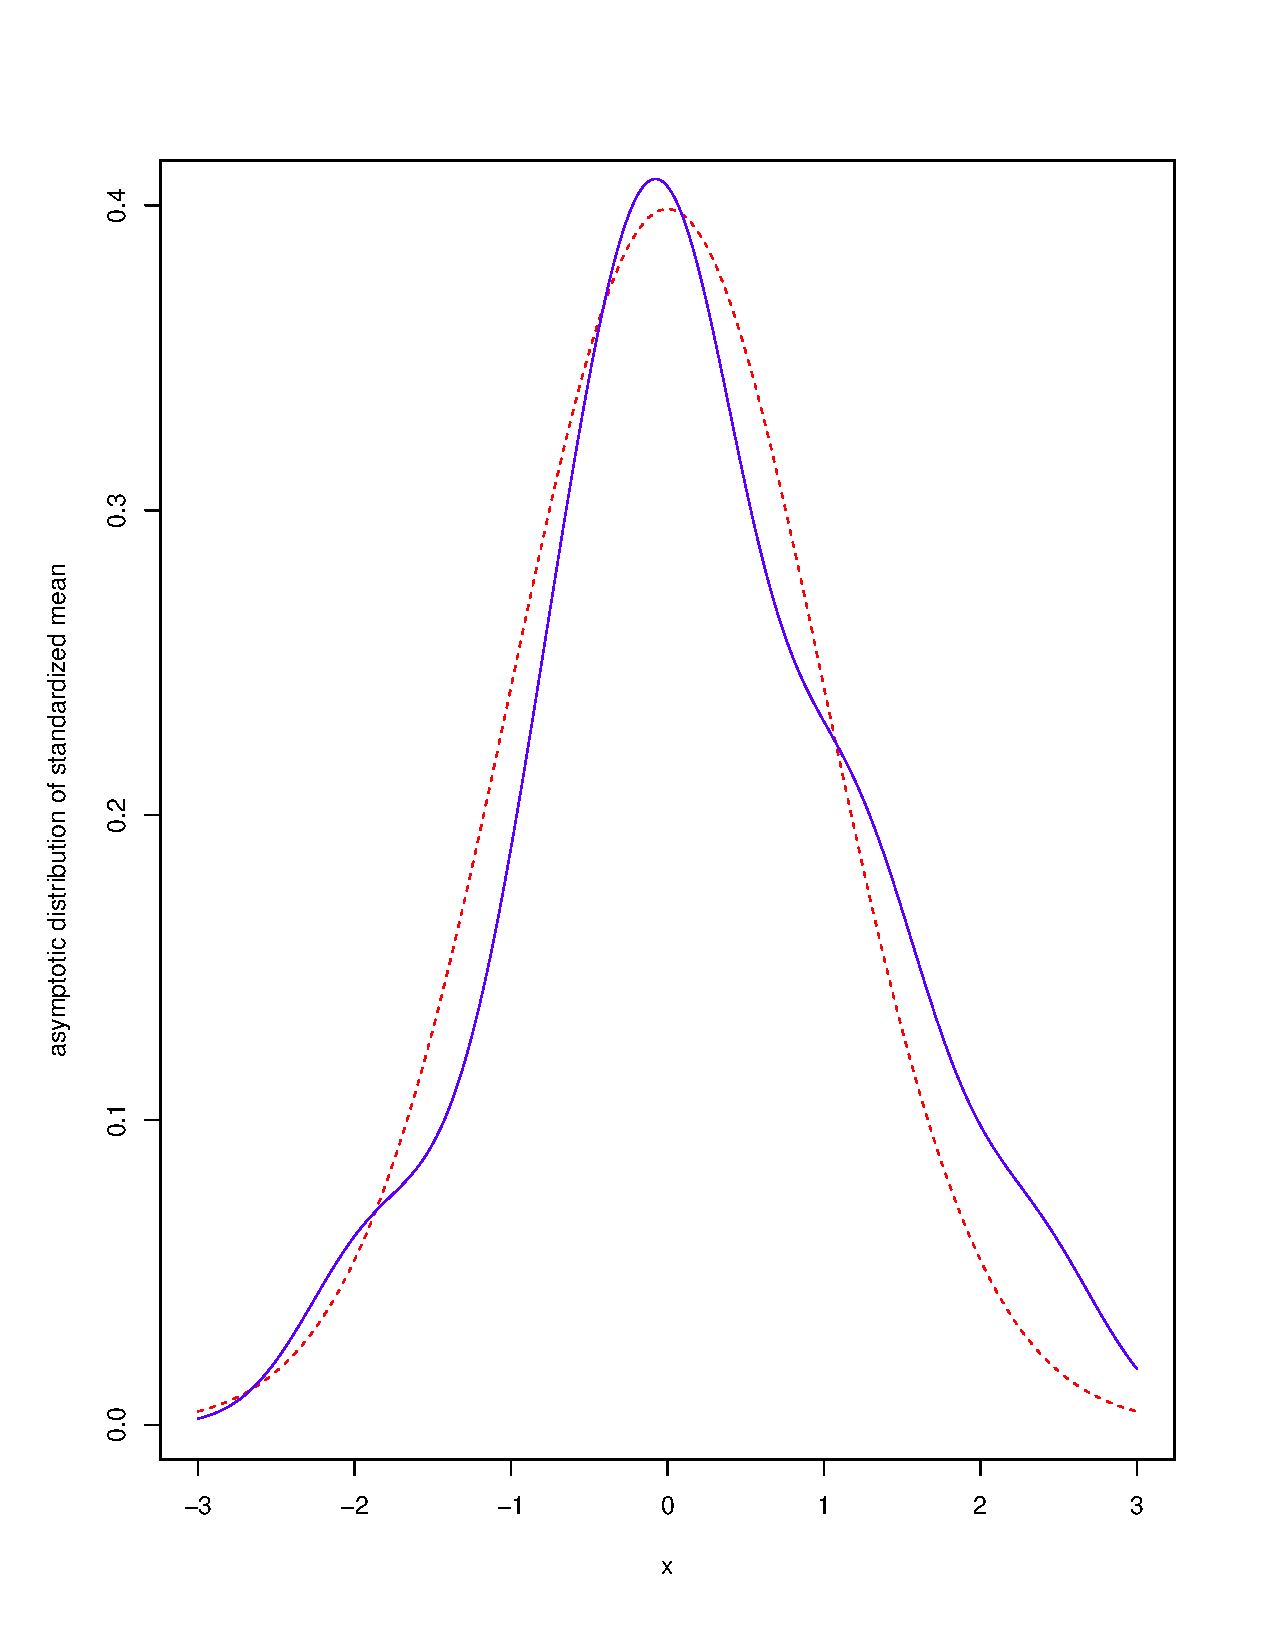
\includegraphics[height=13cm,width=13cm]{pictures/sequential-search-asymtotic-behaviour-of-standardized-means.pdf}
\caption{Plot of standardized means}
\label{fig:sequential-search-standardized-means}
\end{figure}

Also we've build a second plot with a regression of the sampling means in
\autoref{fig:sequential-search-means-regression}. The red line is
drawn after computing the intercept and the coefficient using an
hybrid model. Our attempt to explain the data consists of a mixture up
to the second degree, as follow:
\begin{displaymath}
  \begin{split}
    dims &= \sum_{i}^{n}{dimensions[i]}\\
    means &= \sum_{i}^{n}{mean[i]}\\
    dim\_squares &= \sum_{i}^{n}{dimensions[i]^2}\\
    mean\_squares &= \sum_{i}^{n}{means[i]^2}\\
    dim\_mean &= \sum_{i}^{n}{means[i] * dimensions[i]}\\
    intercept &= \frac{dim\_squares * means - dims *
      dim\_mean}{n*dim\_squares - dims^2}\\
    coefficient &= \frac{n * dim\_mean - dims * means} {n*dim\_squares-dims^2}
  \end{split}
\end{displaymath}
where $n$ is our $numdimensions$ cited above, hence the red line is
defined as $means = coefficient*dimensions + intercept$. Using an R
interpreter we can see our numerical output:
\begin{lstlisting}
  coefficient = 0.49, intercept = 0.66
  square of correlation index = 0.999
\end{lstlisting}
The regression is almost perfect, hence there exists a strong linear
relation between means and distribution (from a statistical point of
view we can conclude with the following observation: for an increment
of the dimensions of one unit we get an increment of about a half unit
on the number of checks).
\begin{figure}[htb]
\centering
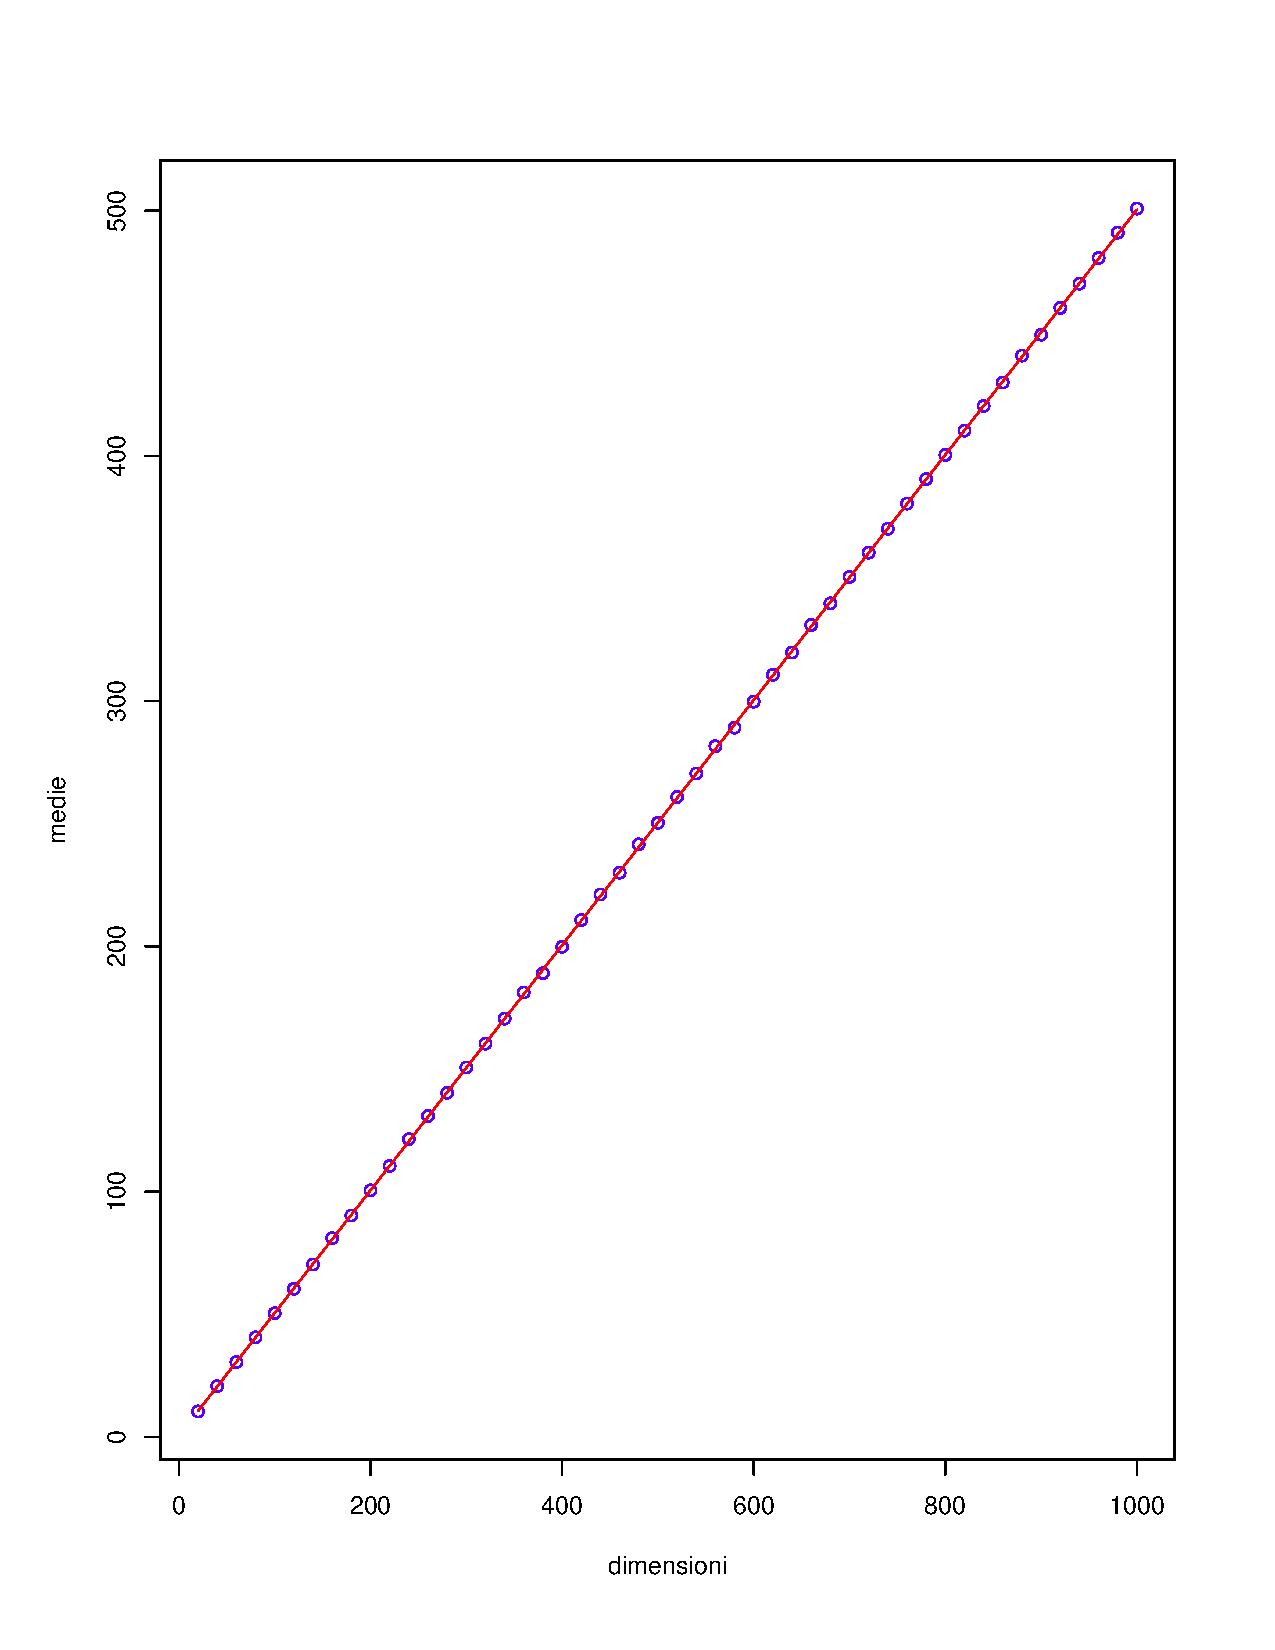
\includegraphics[height=13cm,width=13cm]{pictures/sequential-search-mean-regression-of-sequential-search.pdf}
\caption{Plot of means regression}
\label{fig:sequential-search-means-regression}
\end{figure}


\chapter{Generating binary trees at random}
Explain the project and what we want to accomplish.

\section{Atkinson and Sack algorithm}
Describe briefly the algorithm here.

\section{Implementation using R}

\begin{lstlisting}

  generate.tree <- function(number_of_nodes){

    word_dimension <- 2 * number_of_nodes
    
    universe <- 1:word_dimension
    sample <- sample(universe, size=number_of_nodes)
    w = rep(0, word_dimension)
    for (i in 1:word_dimension) {
      w[i] <- ifelse(any(sample == i), 1, -1)
    }
    
    phi=phi(w)
    list(word=w, phi=phi, as_brackets = brackets_of_word(phi))
  }

  split.word <- function(w){
    if(length(w) == 0){
      return(list(u=c(), v=c()))
    }
    
    u_index_set <- 1:match(0, cumsum(w))
    list(u=w[u_index_set], v=w[-u_index_set])
  }

  phi <- function(w){
    if(length(w) == 0){
      return(w)
    }
    
    split <- split.word(w) 
    
    if(all(cumsum(split$u) > -1)){
      return (c(split$u, phi(split$v)))
    }
    else{
      t = split$u[-c(1, length(split$u))]
      return (c(1, phi(split$v), -1, -t))
    }
  }
\end{lstlisting}

\part{Algorithms part}

\chapter{Divide et impera}
Put here some exercises on some topics of interest.

\chapter{Appendix}

\section{Original article about random binary trees generation}

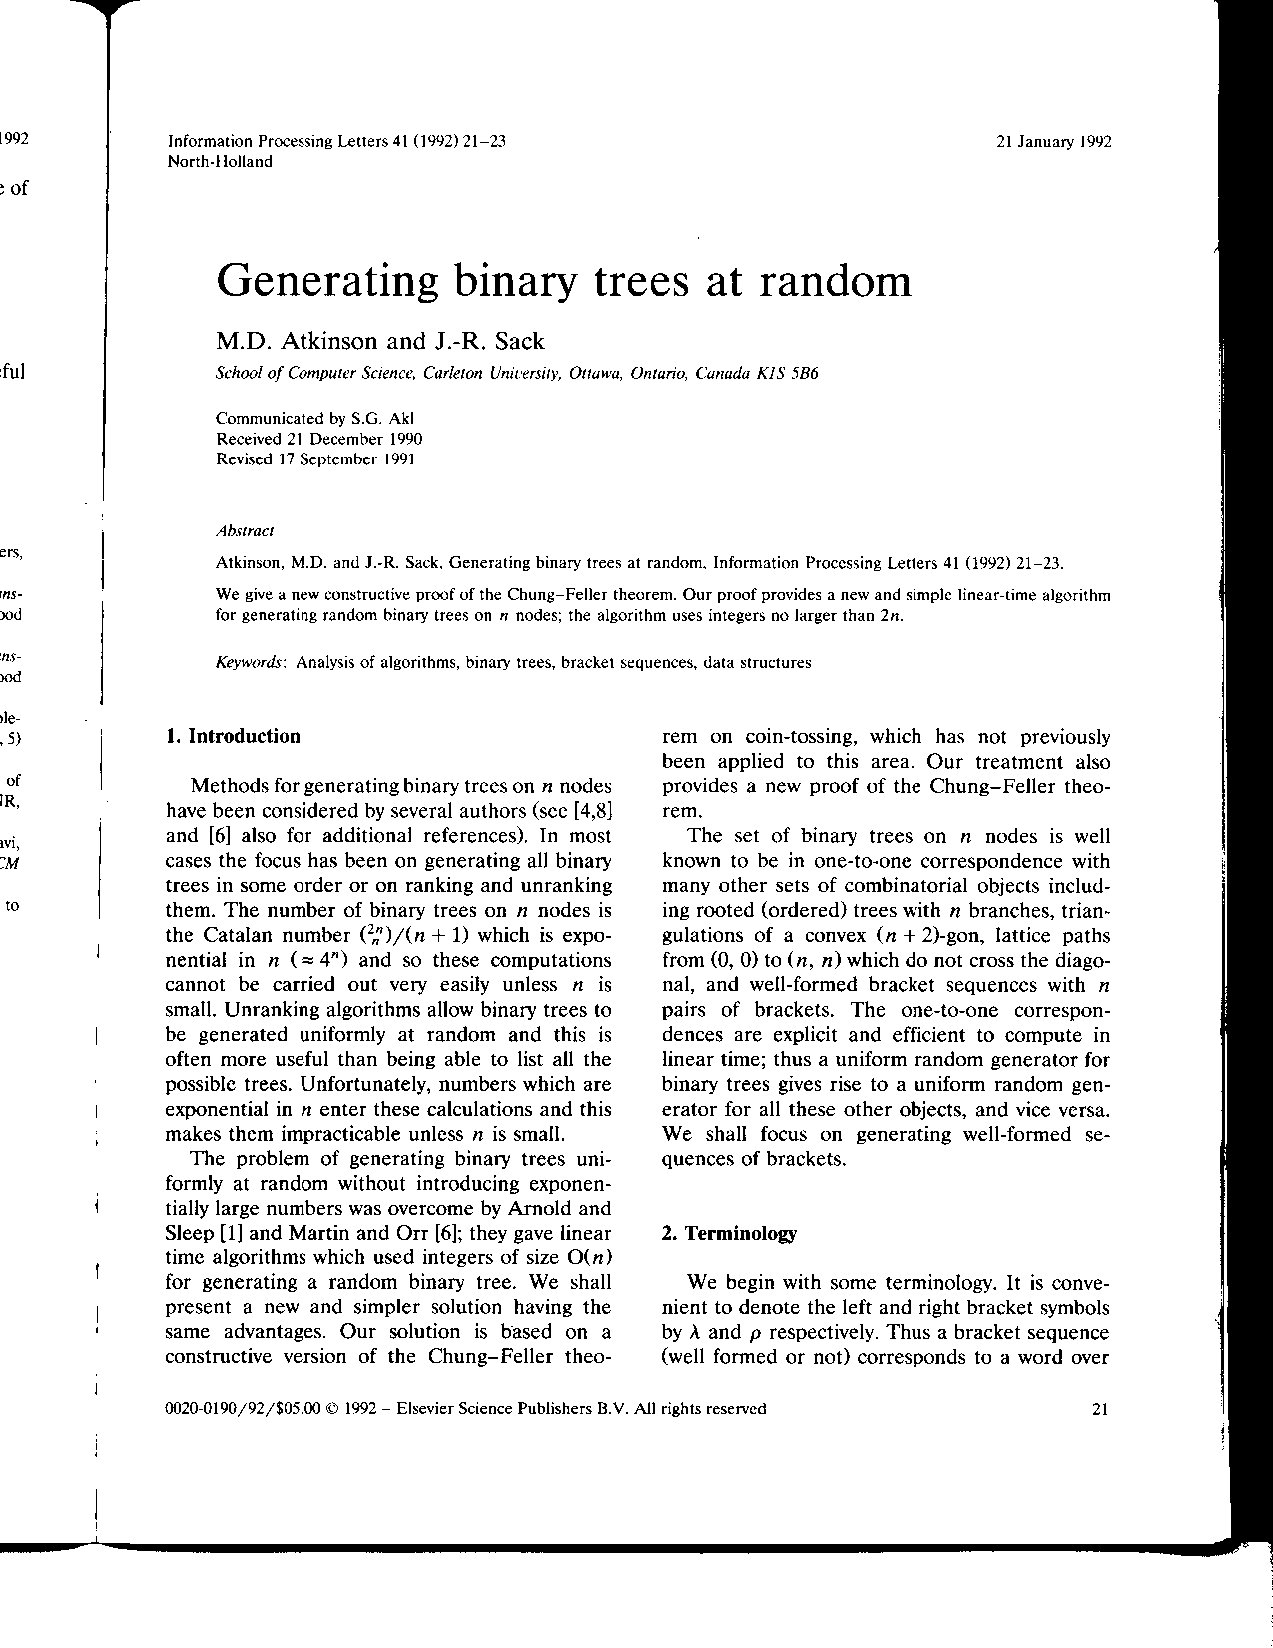
\includepdf[pages={-}]{atkinson-sack-original-article.pdf}

% \section{Full code for random binary trees generation}
% The following block contains the functions written in \emph{R} to
% implement the algorithms related to the generation of binary
% trees. Those functions allow to generate the outputs attached in the
% previous chapters:
% \lstinputlisting{random-trees-generation/generator.R}

% \section{Full code for trees analysis and dot representation}
% The following block contains the functions written in \emph{OCaml} to
% implement the algorithms related to the analysis of the generated
% trees and its dot representation:
% \lstset{language=ML}
% \lstinputlisting{trees-generation-ocaml/main.ml}






\end{document} 
